\documentclass[a4paper, 12pt, final, garamond]{book}
\usepackage{cours-preambule}

\raggedbottom

\makeatletter
\renewcommand{\@chapapp}{\'Electrocin\'etique -- chapitre}
\makeatother

\begin{document}
\setcounter{chapter}{6}

\chapter{Correction du TD}

\section{Filtrage et spectres}
\begin{enumerate}
    \item Sur la figure deux, les basses fréquences sont globalement conservées,
        et les fréquences à partir de \SI{3}{kHz} sont fortement atténuées voire
        coupées~: \textbf{c'est un passe-bas}.
    \item Sur la figure trois, seules les fréquences entre 3 et \SI{4}{kHz} sont
        gardées, les fréquences supérieures ou inférieures sont coupées~:
        \textbf{c'est un passe-bande}.
    \item Sur la figure quatre, on ne distingue pas de relation simple vue en
        cours~; on remarque de plus que de nouvelles fréquences apparaissent, ce
        qui n'est pas le cas dans le filtrage linéaire~: c'est un \textbf{filtre
        non-linéaire}.
\end{enumerate}

\section{Filtre avec une bobine}
\begin{enumerate}
    \item À basses fréquences, $\abs{\ul{Z}_L} \xrightarrow[\w\rightarrow0]{} 0$, donc
        $H(\w) \xrightarrow[\w\rightarrow0]{} 0$. À hautes fréquences,
        $\abs{\ul{Z}_L} \xrightarrow[\w\rightarrow\infty]{} \infty$, donc
        $H(\w) \xrightarrow[\w\rightarrow\infty]{} 1$~: \textbf{c'est un
        passe-haut}.
    \item On fait un pont diviseur de tension~:
        \begin{gather*}
            \ul{u_s} = \frac{\jlw}{R + \jlw}\ul{u_e}
            \Leftrightarrow
            \frac{\ul{u_s}}{\ul{u_e}} = \ul{H} =
            \cancel{\frac{R}{R}}\times\frac{\jj\w\frac{L}{R}}{1 + \jj\w
            \frac{L}{R}}\\
            \Leftrightarrow
            \boxed{\ul{H}(\jj\w) = H_0 \frac{\jj\frac{\w}{\w_c}}{1 +
            \jj\frac{\w}{\w_c}}}
            \qavec
            \boxed{H_0 = 1
            \qet
            \w_c = \frac{R}{L} = \SI{1e5}{rad.s^{-1}}}
        \end{gather*}
    \item $1 + \jj \frac{\w}{\w_c} \underset{\w \ll \w_c}{\sim} 1$, et donc
        \begin{gather*}
            \ul{H}(\jj\w) \underset{\w\ll\w_c}{\sim} \jj \frac{\w}{\w_c}
            \Leftrightarrow
            \boxed{G_{\rm dB} = 20\log \left( \abs{\ul{H}} \right)
            \underset{\w\ll\w_c}{\sim} 20\log x}
        \end{gather*}
        d'où la pente de \SI{20}{dB/décade}.
    \item On trouve le spectre de sortie en multipliant chaque amplitude
        d'entrée par le module de la fonction de transfert pour avoir
        l'amplitude de sortie. \textbf{Attention, pulsation $\neq$ fréquence}.
        On a
        \[\abs{\ul{H}(f)} = \frac{\dfrac{2\pi f}{\w_c}}{\sqrt{1 +
                    \left( \dfrac{2\pi f}{\w_c} \right)^2}}\]
        \begin{itemize}
            \item $H(f_1) \approx \num{6.3e-3}$~: le fondamental est
                complètement atténué, il ne reste que \num{0.6}\% de son
                amplitude initiale~;
            \item $H(f_2) \approx \num{6.3e-2}$~: l'harmonique $f_2$ est
                fortement atténué, il n'en reste que 6\%~;
            \item $H(f_3) \approx \num{0.99}$~: l'harmonique $f_3$ est
                pratiquement entièrement conservé.
        \end{itemize}
\end{enumerate}

\section{Lecture de diagrammes de \textsc{Bode}}

Pour faciliter la rédaction on note $e(t) = e_0 + e_1 (t) + e_{10} (t) + e_{100}
(t)$, et de même pour le signal de sortie $s$. Ainsi, par linéarité, chaque
composante $e_n$ du signal d'entrée donne une composante $s_n$ au signal de
sortie.
\begin{itemize}
    \item Filtre 1~: d'après l'allure du diagramme de \textsc{Bode}, il s'agit d'un
        filtre passe-haut, de fréquence de coupure $f_c$ de l'ordre de
        \SI{10}{kHz}. Reconstruisons le signal de sortie~:
        \begin{itemize}
            \item Le terme constant $e_0$ est complètement coupé par le filtre,
                donc $s_0 = 0$.
            \item L'harmonique de fréquence $f$ est atténuée de \SI{40}{dB} et
                peut donc être négligée dans le signal de sortie (\SI{40}{dB}
                correspond à une division de l'amplitude par 100), soit $s_1 (t)
                \ll$ autres harmoniques de $s(t)$.
            \item L'harmonique de fréquence $10f$ est atténuée de \SI{10}{dB},
                soit \[S = 10^{-10/20} E = 10^{-1/2} E \approx \num{0,3}E\] et
                elle est également déphasée d'environ $+\pi/2$. Ainsi \[s_{10}
                (t) \approx \num{0,3}E \cos(10\wt + \pi/4 + \pi/2)\]
            \item L'harmonique de fréquence $100f$ n'est presque pas atténuée ni
                déphasée, donc $s_{100} (t) \approx e_{100} (t)$. Au final, on
                obtient le signal de sortie $s(t)$ suivant~:
        \end{itemize}
\end{itemize}

\[\boxed{
    s(t) \approx
    \num{0,3}E_0 \cos \left(10\wt + \frac{3\pi}{4}\right) +
    E_0 \cos \left(100\wt - \frac{\pi}{3}\right)
}\]

\begin{itemize}
    \item Filtre 2~: d'après l'allure du diagramme de \textsc{Bode}, il s'agit d'un
        filtre \textbf{passe-haut}, de fréquence de coupure $f_c$ de l'ordre de
        \SI{0.1}{kHz}. De la même manière que pour le fitre 1, on détermine que~:
\end{itemize}

\[\boxed{
    s(t) \approx
    E_0 \cos (\wt) + E_0 \cos \left(10\wt + \frac{\pi}{4}\right) +
    E_0 \cos \left(100\wt - \frac{\pi}{3}\right)
}\]
\begin{itemize}
    \item Filtre 3~: d'après l'allure du diagramme de \textsc{Bode}, il s'agit d'un
        filtre \textbf{coupe-bande}, la bande coupée étant proche de
        \SI{1}{kHz}. Ainsi seule l'harmonique $e_1(t)$ est coupée (soit $s_1 =
        0$). Les autres composantes harmoniques du signal d'entrée, y compris la
        composante continue, sont de fréquences suffisamment différentes de la
        fréquence coupée pour n'être ni atténuée ni déphasée. La signal de
        sortie $s(t)$ s'écrit donc sous la forme~:
\end{itemize}

\[\boxed{
    s(t) =
    E_0 +
    E_0 \cos \left(10\wt - \frac{\pi}{4}\right) +
    E_0 \cos \left(100\wt - \frac{\pi}{3}\right)
}\]
\begin{itemize}
    \item Filtre 4~: d'après l'allure du diagramme de \textsc{Bode}, il s'agit
        d'un filtre \textbf{passe-bas}, de fréquence de coupure $f_c$ de l'ordre
        de \SI{0.1}{kHz}. Le terme constant $e_0$ passe au travers du filtre
        sans être modifié. Les termes suivants sont de fréquence suffisamment
        supérieure à la fréquence de coupure pour que le diagramme de
        \textsc{Bode} puisse être approximé par son asymptote. On peut alors
        déterminer le signal de sortie comme dans le cas du premier filtre, mais
        il y a plus simple~! Comme le filtre est d'ordre 1 (une seule asymptote
        de pente \SI{-20}{dB/décade}, alors il se comporte comme un intégrateur
        pour les signaux de fréquence supérieure à sa fréquence de coupure. En
        déduire le signal de sortie est donc très simple~:
\end{itemize}

\[s(t) =
    E_0 +
    \frac{\w_c}{\w}E_0\sin(\wt) +
    \frac{\w_c}{10\w}\sin \left( 10\wt + \frac{\pi}{4} \right) +
    \frac{\w_c}{100\w} \sin \left( 100\wt - \frac{\pi}{3} \right)
\]
\begin{itemize}
    \item{}
    En écrivant le signal en termes de cosinus, on obtient~:
\end{itemize}
\[\boxed{
    s(t) = 
    E_0 +
    \frac{\w_c}{\w}E_0\cos\left(\wt - \frac{\pi}{2}\right) +
    \frac{\w_c}{10\w}\cos \left( 10\wt - \frac{\pi}{4} \right) +
    \frac{\w_c}{100\w} \cos \left( 100\wt - \frac{5\pi}{6} \right)
}\]

\section{Filtre de \textsc{Wien}}
\begin{enumerate}
    \item Dans la limite très hautes fréquences, les condensateurs sont
        équivalents à des fils, donc $\ul{S} = 0$. Dans la limite très basses
        fréquences, les condensateurs sont cette fois équivalents à des
        interrupteurs ouverts. Aucun courant ne circule dans les résistances, et
        on a donc également $\ul{S} = 0$. Selon toute vraisemblance, c'est donc
        un filtre \textbf{passe-bande}.
    \item Notons $\ul{Z}$ l'impédance et $\ul{Y}$ l'admittance de l'association
        RC parallèle. En utilisant cette impédance, on reconnaît un pont
        diviseur de tension~:
        \begin{gather*}
            \ul{H} = \frac{\ul{S}}{\ul{E}} = \frac{\ul{Z}}{R + \dfrac{1}{\jj
            C\w} + \ul{Z}}
            \Leftrightarrow
            \ul{H}
                = \frac{1}{1 + \left(R + \dfrac{1}{\jj C\w}\right)\ul{Y}}
                = \frac{1}{1 + \left(R + \dfrac{1}{\jj C\w}\right)\left(
                    \dfrac{1}{R} + \jj C\w\right)}\\
            \Leftrightarrow
            \boxed{\ul{H} = \frac{1}{3+\jj\left(RC\w - \dfrac{1}{RC\w}\right)}}
        \end{gather*}
    \item En factorisant par 3 et en utilisant les notations introduites dans
        l'énoncé, on trouve
        \begin{gather*}
            \ul{H}
                = \frac{1/3}{1 + \dfrac{\jj}{3} \left( x - \dfrac{1}{x} \right)}
            \Leftrightarrow
            \boxed{
            \ul{H} = \frac{H_0}{1 + \jj Q \left( x - \dfrac{1}{x} \right)}}
            \qavec
            \boxed{
            \left\{
                \begin{array}{rcl}
                    H_0 & = & 1/3\\
                    Q & = & 1/3
                \end{array}
            \right.
            }
        \end{gather*}
    \item Le gain en amplitude du filtre est défini par
        \[G = \abs{\ul{H}} = \frac{H_0}{\sqrt{1 + Q^2 \left( x - \dfrac{1}{x}
        \right)^2}}\]
        Il est maximal lorsque le dénominateur est minimal, c'est-à-dire lorsque
        le terme entre parenthèses s'annule. Cela correspond à $x=1$, d'où le
        gain maximal $\mathbf{G_{\max} = 1/3}$. \bigbreak
        Le gain \textbf{en décibels} du filtre est défini par
        \[G_{\rm dB} = 20\log(\abs{\ul{H}})\]
        et on trouve donc $\mathbf{G_{\rm dB, max} = 20\log(1/3) =
        \SI{-9.5}{dB}}$. De plus, en $x = 1$ la fonction de transfert est
        réelle, donc son argument est nul~: à la pulsation $\w_0$, la sortie et
        l'entrée ne sont donc pas déphasées.
    \item Dans la limite très basses fréquences, la fonction de transfert est
        équivalente à
        \[\ul{H}
            \underset{x\rightarrow0}{\sim} \frac{H_0}{-\jj Q/x}
            = \jj \frac{H_0}{Q} x
            \qdonc
            \left\{
                \begin{array}{rcl}
                    G_{\dB} & = & 20\log\abs{\ul{H}}
                    \underset{x\rightarrow0}{\sim} 20 \log x\\
                    \f & = & \arg \ul{H} = \frac{\pi}{2}
                \end{array}
            \right.
        \]
        De même, dans la limite très hautes fréquences, on a
        \[\ul{H}
            \underset{x\rightarrow\infty}{\sim} \frac{H_0}{\jj Qx}
            = -\jj \frac{H_0}{Q} \frac{1}{x}
            \qdonc
            \left\{
                \begin{array}{rcl}
                    G_{\dB} & = & 20\log\abs{\ul{H}}
                    \underset{x\rightarrow0}{\sim} -20 \log x\\
                    \f & = & \arg \ul{H} = -\frac{\pi}{2}
                \end{array}
            \right.
        \]

        Ainsi, le diagramme de \textsc{Bode} asymptotique en gain compte
        \textbf{deux asymptotes de pentes $\mathbf{\pm\SI{20}{dB/décade}}$
        passant par $\mathbf{G_{\dB} = 0}$ pour $\mathbf{x=1}$}, alors que le
        diagramme asymptotique en phase compte \textbf{deux asymptotes
        horizontales de hauteurs $\mathbf{\pm \pi/2}$}. \bigbreak
        Pour tracer l'allure du diagramme réel, on utilise en plus les résultats
        de la question précédente qui indique que la courbe réelle passe par
        $G_{\dB} = \SI{-9.5}{dB}$ en $x=1$, alors que la courbe de phase réelle
        passe par $0$ en $x=1$~; d'où les diagrammes ci-dessous.

        \begin{center}
            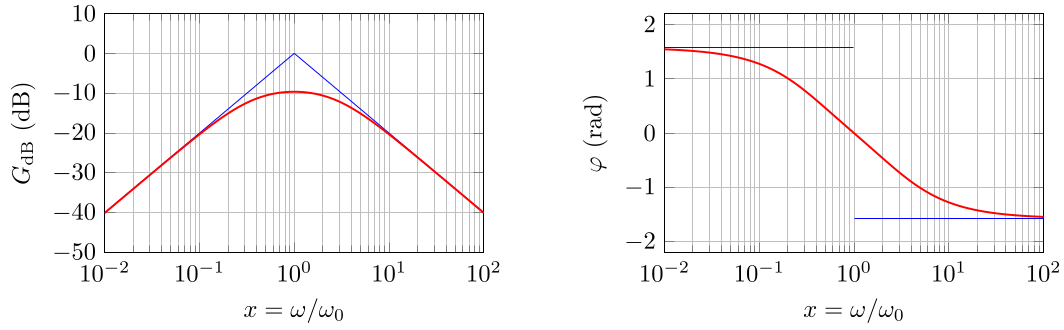
\includegraphics[width=\linewidth]{wien_bode}
        \end{center}
    \item Numériquement, on trouve $\w_0 = \SI{2.0e3}{rad.s^{-1}}$. Comme le
        diagramme de \textsc{Bode} réel n'est pas donné dans l'énoncé, on peut
        au choix utiliser la fonction de transfert ou raisonner sur le diagramme
        asymptotique. Étudions le signal de sortie du filtre associé à chaque
        composante du signal d'entrée~:
        \begin{itemize}
            \item Le terme continu est complètement coupé par le filtre~;
            \item Le terme de pulsation $\w = \w_0/10$ se trouve une décade
                en-dessous de la pulsation propre~: avec le diagramme
                asymptotique il est donc atténué de \SI{20}{dB}, ce qui
                correspond à un facteur 10 en amplitude, et déphasé d'environ
                \SI{1.2}{rad} si le diagramme réel tracé~;
            \item Le terme de pulsation $10\w = \w_0$ est à la pulsation propre
                du filtre~: il n'est pas déphasé mais seulement atténué d'un
                facteur 1/3 (gain maximal)~;
            \item Le terme à la pulsation $100\w = 10\w_0$ est une décade
                au-dessus de la pulsation propre~: il est atténué comme le
                premier terme d'un facteur 10 en amplitude, et déphasé d'environ
                \SI{-1.2}{rad}. Ainsi,
        \end{itemize}
\end{enumerate}
\[\boxed{
    s(t) =
        \frac{E_0}{10}\cos (\wt - \num{1.2}) +
        \frac{E_0}{3}\cos(10\wt) +
        \frac{E_0}{10}\cos (100\wt + \num{1.2})
}\]

\section{Filtre ADSL}
\begin{enumerate}
    \item On isole les signaux téléphoniques avec un \textbf{filtre passe-bas},
        et les signaux informatiques avec un \textbf{filtre passe-haut}. La
        fréquence de coupure doit être à la fois nettement supérieure aux
        fréquences téléphoniques et nettement plus faible que les fréquences
        informatiques~: on prendra donc \fbox{$f_0 = \SI{10}{kHz}$}.
    \item ~

        \vspace{-24pt}
        \begin{minipage}{0.45\linewidth}
            En basses fréquences ($\w \longrightarrow 0$), les bobines se
            comportent comme des fils, soit
            \begin{center}
                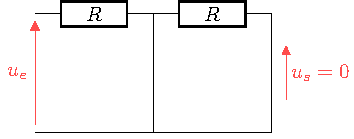
\includegraphics[width=\linewidth]{adsl_bf}
            \end{center}
        \end{minipage}
        \hfill
        \vrule
        \hfill
        \begin{minipage}{0.45\linewidth}
            En hautes fréquences ($\w \longrightarrow \infty$), les bobines se
            comportent comme des interrupteurs ouverts, soit
            \begin{center}
                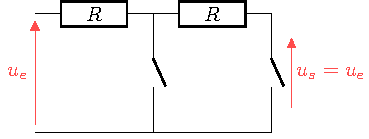
\includegraphics[width=\linewidth]{adsl_hf}
            \end{center}
        \end{minipage}
        Ainsi, le signal de sortie est non nul pour les hautes fréquences, et
        négligeable pour les basses fréquences~: c'est un \textbf{filtre
        passe-haut}. Il permettra d'obtenir les signaux informatiques.
    \item Pour exprimer $u_s$ en fonction de $u_e$, on peut faire un premier
        pont diviseur de tension pour exprimer $u_s$ en fonction de $u_{AB}$ du
        milieu~; puis avec une impédance équivalente à l'ensemble des 3 dipôles
        de droite, on refait un pont diviseur de tension pour avoir $u_{AB}$ en
        fonction de $u_e$, et on combine.
        \begin{center}
            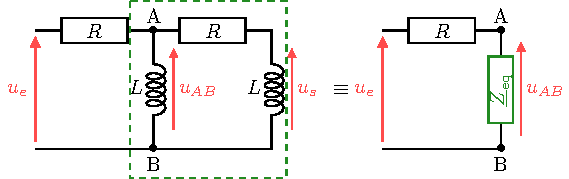
\includegraphics[width=0.6\linewidth]{adsl_equiv}
        \end{center}
        On a donc d'abord~:
        \begin{gather*}
            \Uu_s = \frac{\Zu_L}{\Zu_L + \Zu_R}\Uu_{AB}
            \Leftrightarrow
            \Uu_s = \frac{\jlw}{\jlw + R}\Uu_{AB}
        \end{gather*}
        On aura donc ensuite~:
        \begin{gather*}
            \Uu_{AB} = \frac{\Zu_{\eq}}{\Zu_{\eq} + \Zu_R}\Uu_e
            \Leftrightarrow
            \Uu_{AB} = \frac{1}{1+\Zu_R\Yu_{\eq}}\Uu_e
        \end{gather*}
        On calcule alors $\Yu_{\eq}$~:
        \begin{gather*}
            \Yu_{\eq} = \frac{1}{\jlw} + \frac{1}{R+\jlw}
        \end{gather*}
        Et on combine~:
        \begin{gather*}
            \Uu_s =
                \frac{\jlw}{R+\jlw}\times\frac{1}{1+\Zu_R\Yu_{\eq}}\Uu_e
            \Leftrightarrow
            \Uu_s =
                \frac{\jlw}{R + \jlw + R \left( \dfrac{R+\jlw}{\jlw} + 1
                \right)}\times {\color{Red} \frac{\jlw}{\jlw}}\Uu_e\\
            \Leftrightarrow
            \Uu_s =
                \frac{-(L\w)^2}{R^2 + 3\jj RL\w - (L\w)^2}\Uu_e
            \Leftrightarrow
            \Uu_s =
                {\color{red}\cancel{\frac{R^2}{R^2}}}
                \frac{- \left( \dfrac{L}{R}\w \right)^2}{1 + 3\jj \dfrac{L}{R}\w
                - \left( \dfrac{L}{R}\w \right)^2}
        \end{gather*}
        Ainsi, en divisant par $\Uu_e$ pour avoir la fonction de transfert, on
        a~:
        \begin{gather*}
            \boxed{\Hu = \frac{-x^2}{1-x^2+3\jj x}}
            \qavec
            \boxed{\w_0 = \frac{R}{L}}
        \end{gather*}
    \item Pour $x \gg 1$, les termes en $x^2$ l'emportent sur les autres termes
        au numérateur et au dénominateur, et la fonction de transfert devient
        $\Hu \underset{x\rightarrow\infty}{\sim} 1$, donc \fbox{$G_{\dB} = 0$}
        et \fbox{$\f = 0$} (réel positif). \bigbreak
        Pour $x \ll 1$, les termes en $x$ sont négligeables devant $1$ au
        dénominateur, et on garde le numérateur~: la fonction de transfert
        devient donc $\Hu \underset{x\rightarrow0}{\sim} -x^2$, donc
        \fbox{$G_{\dB} \underset{x\rightarrow0}{\sim} 40\log(x)$} (pente de
        40\,\dB/décade), et \fbox{$\f = -\pi$} (réel négatif). \bigbreak
        Pour $x = 1$, on trouve $\Hu(1) = \jj/3$ donc \fbox{$G_{\dB}(1) =
        20\log(1/3) = \SI{-9.5}{dB}$}, et \fbox{$\f(1) = \pi/2$} (imaginaire pur).
\end{enumerate}
\begin{center}
    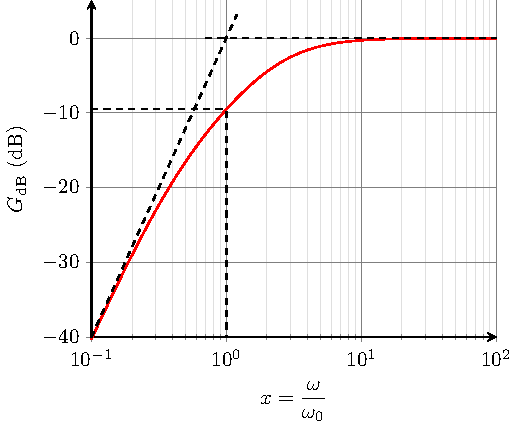
\includegraphics[width=.48\linewidth]{adsl_bode-gain}
    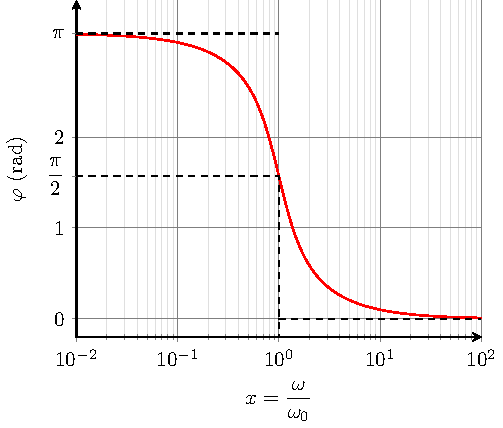
\includegraphics[width=.48\linewidth]{adsl_bode-phase}
\end{center}
\begin{enumerate}[resume]
    \item{} Il n'y a pas de pic de résonance car le facteur de qualité $Q$ est
        plus petit que $1/\sqrt{2}$.
    \item La fréquence de coupure est $f_0 = \DS \frac{\w_0}{2\pi} =
        \frac{R}{2\pi L}$~; on doit donc prendre
        \begin{gather*}
            \boxed{L = \frac{R}{2\pi f_0}}
            \qavec
            \left\{
                \begin{array}{rcl}
                    R & = & \SI{100}{\Omega}\\
                    f_0 & = & \SI{10}{kHz}
                \end{array}
            \right.\\
            \mathrm{A.N.~:}\quad
            \boxed{L = \SI{1.6}{mH}}
        \end{gather*}
\end{enumerate}

\end{document}
